%% LyX 2.2.1 created this file.  For more info, see http://www.lyx.org/.
%% Do not edit unless you really know what you are doing.
\documentclass[english,12pt]{article}
\usepackage[T1]{fontenc}
\usepackage[latin9]{inputenc}
\usepackage{float}
\usepackage{booktabs}
\usepackage{mathtools}
\usepackage{amsmath}
\usepackage{amsthm}
\usepackage{amssymb}
\usepackage{graphicx}

\makeatletter

%%%%%%%%%%%%%%%%%%%%%%%%%%%%%% LyX specific LaTeX commands.
%% Because html converters don't know tabularnewline
\providecommand{\tabularnewline}{\\}
\floatstyle{ruled}
\newfloat{algorithm}{tbp}{loa}
\providecommand{\algorithmname}{Algorithm}
\floatname{algorithm}{\protect\algorithmname}

%%%%%%%%%%%%%%%%%%%%%%%%%%%%%% Textclass specific LaTeX commands.
\theoremstyle{plain}
\newtheorem{thm}{\protect\theoremname}[section]
\theoremstyle{definition}
\newtheorem{defn}[thm]{\protect\definitionname}
\theoremstyle{remark}
\newtheorem{rem}[thm]{\protect\remarkname}
\theoremstyle{plain}
\newtheorem{prop}[thm]{\protect\propositionname}
\ifx\proof\undefined
\newenvironment{proof}[1][\protect\proofname]{\par
\normalfont\topsep6\p@\@plus6\p@\relax
\trivlist
\itemindent\parindent
\item[\hskip\labelsep\scshape #1]\ignorespaces
}{%
\endtrivlist\@endpefalse
}
\providecommand{\proofname}{Proof}
\fi
\theoremstyle{definition}
\newtheorem{example}[thm]{\protect\examplename}

%%%%%%%%%%%%%%%%%%%%%%%%%%%%%% User specified LaTeX commands.
\usepackage[margin=1in]{geometry}
\usepackage{tikz}
\usetikzlibrary{arrows,decorations.pathreplacing,shapes}

\makeatother

\usepackage{babel}
\usepackage{listings}
\providecommand{\definitionname}{Definition}
\providecommand{\examplename}{Example}
\providecommand{\propositionname}{Proposition}
\providecommand{\remarkname}{Remark}
\providecommand{\theoremname}{Theorem}
\renewcommand{\lstlistingname}{Listing}

\begin{document}

\title{Math 525: Lecture 24}

\date{April 12, 2018}
\maketitle

\section{Conditional distribution and expectations}

Let $X$ and $Y$ be random variables. If the event $\{X=x\}$ occurs
with positive probability, we can define the \emph{conditional distribution
function} by
\[
F_{Y\mid X}(y\mid x)=\mathbb{P}\left\{ Y\leq y\mid X=x\right\} .
\]
If $Y$ is also integrable, we can also define the \emph{conditional
expectation} of $Y$ given $X=x$:
\[
\mathbb{E}\left[Y\mid X=x\right]=\frac{\mathbb{E}\left[YI_{\{X=x\}}\right]}{\mathbb{P}\left\{ X=x\right\} }.
\]
We saw in a previous class that if in addition to being integrable,
$Y$ is discrete, the above simplifies:
\[
\mathbb{E}\left[Y\mid X=x\right]=\frac{\sum_{n}y_{n}\mathbb{P}\left\{ Y=y_{n},X=x\right\} }{\mathbb{P}\left\{ X=x\right\} }=\sum_{n}y_{n}\mathbb{P}\left\{ Y=y_{n}\mid X=x\right\} .
\]

However, when $X$ has a continuous distribution, the event $\{X=x\}$
has probability zero. While it is possible to define $\mathbb{E}[Y\mid\cdot\,]$
in a general way that avoids this issue, doing so requires knowledge
of some concepts from measure theory (e.g., Radon-Nikodym derivatives).
Instead of working in the most general setting, we will instead tackle
the case in which $X$ and $Y$ admit a joint density $f_{XY}$.

To motivate our definition of conditional distribution in this setting,
suppose events of the form $\{x\leq X\leq x+h\}$ have positive probability
(where $h>0$) and consider
\[
\mathbb{P}\left(Y\leq y\mid x\leq X\leq x+h\right).
\]
Since $X$ and $Y$ admit a joint density,
\[
\mathbb{P}\left(Y\leq y\mid x\leq X\leq x+h\right)=\frac{\mathbb{P}\left\{ Y\leq y,x\leq X\leq x+h\right\} }{\mathbb{P}\left\{ x\leq X\leq x+h\right\} }=\frac{\int_{-\infty}^{y}\int_{x}^{x+h}f_{XY}(u,v)dudv}{\int_{x}^{x+h}f_{X}(u)du}.
\]
If $h$ is small, we expect the above to be approximately
\[
\frac{h\int_{-\infty}^{y}f_{XY}(x,v)dv}{hf_{X}(x)}=\frac{\int_{-\infty}^{y}f_{XY}(x,v)dv}{f_{X}(x)}=\int_{-\infty}^{y}\left(\frac{f_{XY}(x,v)}{f_{X}(x)}\right)dv.
\]
This motivates the definition below.
\begin{defn}
Let $X$ and $Y$ be random variables which admit a joint density
$f_{XY}$. We can define the \emph{conditional density} of $Y$ given
$X=x$ by
\[
f_{Y\mid X}(y\mid x)=\begin{cases}
{\displaystyle \frac{f_{XY}(x,v)}{f_{X}(x)}} & \text{if }f_{X}(x)>0\\
0 & \text{otherwise}.
\end{cases}
\]
The \emph{conditional distribution function} of $Y$ given $X=x$
is
\[
F_{Y\mid X}(y\mid x)=\int_{-\infty}^{y}f_{Y\mid X}(v\mid x)dv.
\]
The \emph{conditional expectation} of $Y$ given $X=x$ is
\[
\mathbb{E}\left[Y\mid X=x\right]=\int_{-\infty}^{\infty}yf_{Y\mid X}(y\mid x)dy.
\]
\end{defn}
\begin{rem}
If $X$ and $Y$ are independent in the above, the conditional density
of $Y$ given $X=x$ should be independent of $X$. Indeed, then
\[
f_{Y\mid X}(y\mid x)=\frac{f_{XY}(x,y)}{f_{X}(x)}=f_{Y}(y).
\]
Let's also verify that the conditional density works as desired. Indeed,
\begin{align*}
\int_{a}^{b}\overbrace{\left(\int_{c}^{d}f_{Y\mid X}(y\mid x)dy\right)}^{\mathbb{P}\left(c<Y\leq d\mid X=x\right)}f_{X}(x)dx & =\int_{a}^{b}\int_{c}^{d}\frac{f_{XY}(x,y)}{f_{X}(x)}f_{X}(x)dydx\\
 & =\int_{a}^{b}\int_{c}^{d}f_{XY}(x,y)dydx\\
 & =\mathbb{P}\left(a<X\leq b,c<Y\leq d\right).
\end{align*}
\end{rem}
\begin{defn}
Suppose $X$ is a discrete random variable or that $X$ and $Y$ admit
a joint density. Suppose $Y$ is integrable, so that the function
$\psi$ given by
\[
\psi(x)=\mathbb{E}\left[Y\mid X=x\right]
\]
is well-defined (if $X$ is discrete, we can safely ignore points
at which $\{X=x\}$). Then, the conditional expectation of $Y$ given
$X$ is
\[
\mathbb{E}\left[Y\mid X\right]\equiv\psi\circ X.
\]
\end{defn}
Unlike the previous definition, we have not specified the value of
$X$ in the conditional expectation. Therefore, unlike $\mathbb{E}\left[Y\mid X=x\right]$
(which is a scalar), $\mathbb{E}\left[Y\mid X\right]$ is itself a
random variable. We now prove what is known as the \emph{tower property
of expectations}:\footnote{Actually, the tower property is more general, applying to the more
general notion of conditional expectation we hinted at before.}
\begin{prop}
Let $X$ and $Y$ be random variables which admit a joint density
$f_{XY}$. Suppose $f_{X}\neq0$. If $Y$ is integrable, then $\mathbb{E}[Y\mid X]$
is also integrable and
\[
\mathbb{E}\left[\mathbb{E}\left[Y\mid X\right]\right]=\mathbb{E}Y.
\]
\end{prop}
\begin{proof}
First, suppose $Y$ is positive. Then,
\begin{align*}
\mathbb{E}\left[\mathbb{E}\left[Y\mid X\right]\right] & =\mathbb{E}\left[\psi(X)\right]\\
 & =\int_{-\infty}^{\infty}\psi(x)f_{X}(x)dx\\
 & =\int_{-\infty}^{\infty}\mathbb{E}\left[Y\mid X=x\right]f_{X}(x)dx\\
 & =\int_{-\infty}^{\infty}\int_{-\infty}^{\infty}yf_{Y\mid X}(y\mid x)dyf_{X}(x)dx\\
 & =\int_{-\infty}^{\infty}\int_{-\infty}^{\infty}y{\displaystyle \frac{f_{XY}(x,y)}{f_{X}(x)}}dyf_{X}(x)dx\\
 & =\int_{-\infty}^{\infty}\int_{-\infty}^{\infty}y{\displaystyle f_{XY}(x,y)}dydx\\
 & =\mathbb{E}\left[Y\right].
\end{align*}
If $Y$ is not positive, we can split it into its positive and negative
parts $Y=Y^{+}-Y^{-}$.
\end{proof}
The tower property also holds for discrete random variables, in which
case the intuition is very easy to understand:
\begin{example}
Consider two bags, labelled $a$ and $b$. We pick bag $a$ with probability
$P$ and bag $b$ with probability $1-p$. We use the random variable
$X$ to indicate which bag we picked (i.e., $X$ takes values in $\{a,b\}$).
Both bags are filled with green and red balls. Define
\[
p_{a}=\frac{\text{\# of green balls in bag }a}{\text{total \# of balls in bag }a}\qquad\text{and}\qquad p_{b}=\frac{\text{\# of green balls in bag }b}{\text{total \# of balls in bag }b}.
\]
From the bag we have chosen, we pick a single ball. Let
\[
Y=\begin{cases}
1 & \text{if we picked a green ball}\\
0 & \text{if we picked a red ball}.
\end{cases}
\]
Then,
\[
\mathbb{E}\left[Y\mid X=a\right]=p_{a}\qquad\text{and}\qquad\mathbb{E}\left[Y\mid X=b\right]=p_{b}.
\]
Therefore,
\[
\mathbb{E}\left[\mathbb{E}\left[Y\mid X\right]\right]=P\left(\mathbb{E}\left[Y\mid X=a\right]\right)+\left(1-P\right)\mathbb{E}\left[Y\mid X=b\right]=Pp_{a}+\left(1-P\right)p_{b}=\mathbb{E}\left[Y\right].
\]

\pagebreak{}
\end{example}

\section{Introduction to Monte Carlo methods}

A Monte Carlo method is any algorithm that exploits the law of large
numbers to compute a (determinstic) quantity. This is best motivated
by example:
\begin{example}
Suppose we want to approximate the value of $\pi$. Recall that for
a (Borel) function $f$, 
\[
\mathbb{E}\left[f(X)\right]=\frac{1}{b-a}\int_{a}^{b}f(x)dx\qquad\text{if }X\sim U[a,b].
\]
The same is true in higher dimensions:
\[
\mathbb{E}\left[f(X,Y)\right]=\frac{1}{d-c}\frac{1}{b-a}\int_{c}^{d}\int_{a}^{b}f(x,y)dxdy\qquad\text{if }X\sim U[a,b]\text{ and }Y\sim U[c,d].
\]
Recall that $\pi$ is the area of a unit circle. That is, letting
$C=\{(x,y)\colon x^{2}+y^{2}\leq1\}$,
\[
\pi=\int_{-1}^{1}\int_{-1}^{1}I_{C}(x,y)dxdy.
\]
\begin{figure}
\begin{centering}
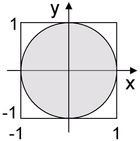
\includegraphics[width=2in]{circle}
\par\end{centering}
\caption{Circle with area $\pi$}
\end{figure}
In other words,
\[
\mathbb{E}\left[I_{C}(X,Y)\right]=\frac{\pi}{4}\qquad\text{where}\qquad X,Y\sim U[-1,1].
\]
Let $X_{n},Y_{n}\sim U[-1,1]$. Then, by the strong law of large numbers,
\[
\lim_{N\rightarrow\infty}\frac{I_{C}(X_{1},Y_{1})+\cdots+I_{C}(X_{N},Y_{N})}{N}=\frac{\pi}{4}\text{ a.s.}
\]
This gives us a very simple algorithm to approximate $\pi$:
\begin{enumerate}
\item Pick a positive integer $N$ and set $S_{N}$ to zero.
\item Generate two (independent) random variables $X$ and $Y$ from the
uniform distribution $U[-1,1]$. If $X^{2}+Y^{2}\leq1$, increment
$S_{N}$ by one.
\item Repeat step (2) $n$ times. Then, $\pi/4\approx S_{N}/N$.
\end{enumerate}
Some MATLAB code for this procedure is given below:

\begin{algorithm}[H]
\begin{lstlisting}[language=Matlab,basicstyle={\footnotesize}]
% Generate (X, Y) pairs
pairs = 2 * rand(2, N) - 1;

% Count which pairs are in the circle
S_N = sum(sum(pairs.^2) <= 1);

pi_approximate = 4 * (S_N / N);
\end{lstlisting}

\caption{Monte Carlo method to approximate $\pi$}
\end{algorithm}
With $N$ equal to 10 million, below are some results of running the
code:

\begin{table}[H]
\centering{}\footnotesize%
\begin{tabular}{cc}
\toprule 
\textbf{Run} & \textbf{Result}\tabularnewline
\midrule
1 & 3.1414432\tabularnewline
2 & 3.1416316\tabularnewline
3 & 3.1418980\tabularnewline
4 & 3.1416388\tabularnewline
5 & 3.1424888\tabularnewline
\bottomrule
\end{tabular}
\end{table}
\end{example}
Even though we used 10 million samples in the above, our approximation
is only accurate up to three significant digits! The slow convergence\footnote{There are much more effective ways to compute $\pi$ (e.g., Chudnovsky
algorithm), but they do not have to do with Monte Carlo.} is explained by the CLT, which says
\[
\frac{1}{\sqrt{N}}\left(\frac{S_{N}}{N}-\frac{\pi}{4}\right)\xrightarrow{\mathcal{D}}\mathcal{N}(0,\sigma)
\]
where $\sigma^{2}=\operatorname{Var}(I_{C}(X,Y))$. With a slight
abuse of notation, we may write
\[
\left|\pi_{\text{approximate}}-\pi\right|=\left|4\frac{S_{N}}{N}-\pi\right|=O\left(\frac{1}{\sqrt{N}}\right)
\]
to represent this fact.
\end{document}
